\documentclass[onecolumn]{article}
\usepackage[spanish]{babel}
\usepackage{caption}
\usepackage{graphicx}
\usepackage{amsmath}
\setlength{\parindent}{0pt}

\author{Josué Villasante}
\title{Medición del tamaño del haz de un laser}

\begin{document}
	\maketitle

	\section{Objetivo}
		El objetivo fue obtener el tamaño del haz del láser utilizando dos procedimientos. El primer procedimiento consistió en utilizar una cuchilla para medir luego de ella como cambia la intensidad a medida esta va bloqueando el haz. El segundo procedimiento utilizó la camara fotográfica para obtener una imagen de la intesidad del haz.

	\section{Resultados}
		De la imagen capturada por una camara (Thorlabs DCU223C) se tomó la fila que presentó la mayor intensidad y esta se ajustó a una gaussiana. 
		$$
		f(x) = \frac{1}{\sigma\sqrt{2\pi}}\exp({-\frac{(x-\mu)^2}{2\sigma^2}})
		$$
		Esto se puede ver en la imagen \ref{cintura}. Los parámetros que se obtuvieron del ajuste fueron $\sigma=45.75$ y $\mu=392.07$. Tomando en cuenta que la altura del sensor son 3.571mm se obtuvo que el diametro del haz utilizando \textit{Full width at half maximum}(FWHM) es 0.50mm y 0.85mm tomando los puntos que son $1/e^2$ veces el máximo.

		\begin{center}
			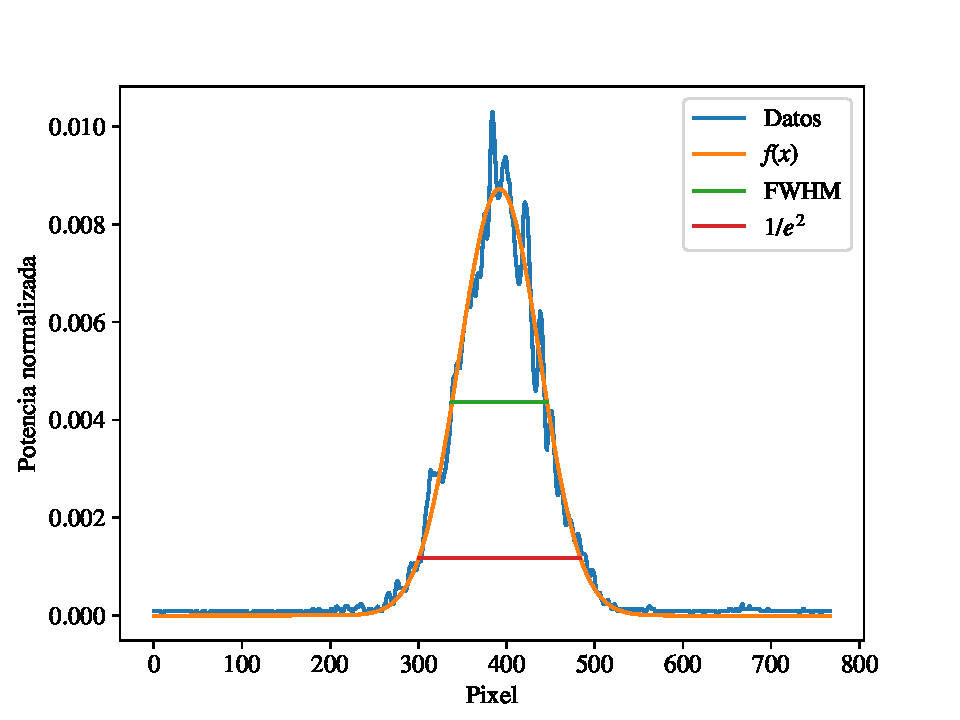
\includegraphics[width=200pt]{img/plot-LaserCintura.pdf}
			\captionof{figure}{Distribución normal ajustada a la potencia normalizada y capturada por una fila de pixeles de la cámara.}
			\label{cintura}
		\end{center}

		Lo mismo se realizó para el haz luego de pasar por la fibra. Los parámetros que se obtuvieron del ajuste fueron $\sigma=97.80$ y $\mu=375.89$. El diametro del haz utilizando FWHM fue 1.07mm y 1.81mm tomando los puntos que son $1/e^2$ veces el máximo.

		\begin{center}
			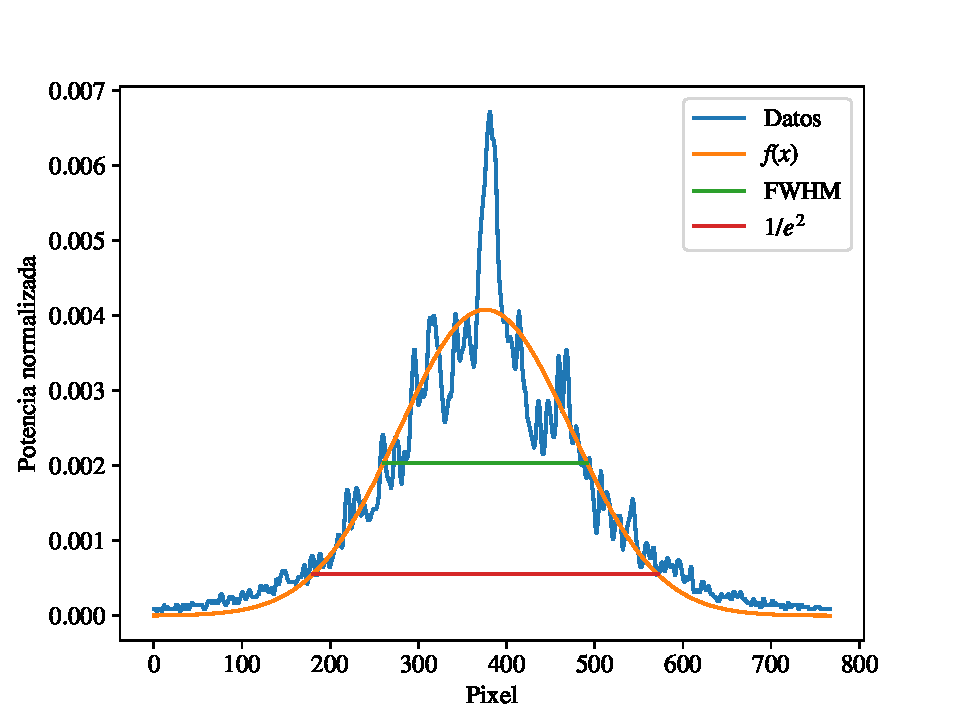
\includegraphics[width=200pt]{img/plot-FibraCintura.pdf}
			\captionof{figure}{Distribución normal ajustada a la potencia normalizada y capturada por una fila de pixeles de la cámara.}
			\label{cintura}
		\end{center}

\end{document}